\documentclass{article}
\usepackage[hidelinks]{hyperref}
\usepackage{apacite}
\usepackage{authblk}
\usepackage{graphicx}
\usepackage{a4wide}
\usepackage{booktabs}
\usepackage{rotating}
\usepackage[nonumberlist]{glossaries}

\bibliographystyle{apacite}
\makeglossaries
\newacronym{MSP}{MSP}{Metagenomic Species Pan-genomes}
\newacronym{HMP}{HMP}{Human Microbiome Project}
\newacronym{CAG}{CAG}{Co-Abundance gene Groups}
\newacronym{CPU}{CPU}{Central Processing Unit}
\newacronym{GPU}{GPU}{Graphical Processing Unit}
\newacronym{MAG}{MAG}{Metagenome-Assembled Genome}
\newacronym{VAE}{VAE}{Variational Auto Encoders}

% For drafts
\usepackage{setspace}
\doublespacing
\usepackage{lineno}
\linenumbers

\title{Advances in Metagenomic Binning for the Reconstruction of Microbial Species}
\author[1*]{Jose Fernando Garcia Guevara}
\author[1*]{Theo Portlock}
\author[1,2]{Adil Mardinoglu}
\author[1]{Mathias Uhlén}
\author[1,2]{Saeed Shoaie}
\affil[1]{Science for Life Laboratory, Royal Institute of Technology (KTH), Stockholm, Sweden.}
\affil[2]{Centre for HostMicrobiome Interactions, Faculty of Dentistry, Oral \& Craniofacial Sciences, King’s College London, London, UK. }

\date{}
\makeglossaries

\begin{document}
\maketitle
\tableofcontents

\printglossaries

\section{Abstract}
New generations of sequencing platforms coupled with numerous bioinformatics tools have led to rapid technological progress in metagenomics to investigate complex microorganism communities.
Nevertheless, a combination of different bioinformatic tools remains necessary to draw conclusions out of microbiota studies.
As sequencing costs have dropped at a rate above 'Moore's law', a greater number of large data sets are being produced than ever before.
Newer algorithms that take advantage of the size of these datasets are continually being developed.
Binning algorithms are defined as the grouping of assembled metagenomic contigs by their genome of origin (\autoref{Fsummary}).
Selecting the most appropriate binning algorithm can be a daunting task and is influenced by many factors.
This review details the current advances in the field of metagenomic binning.

\begin{figure}
\centering
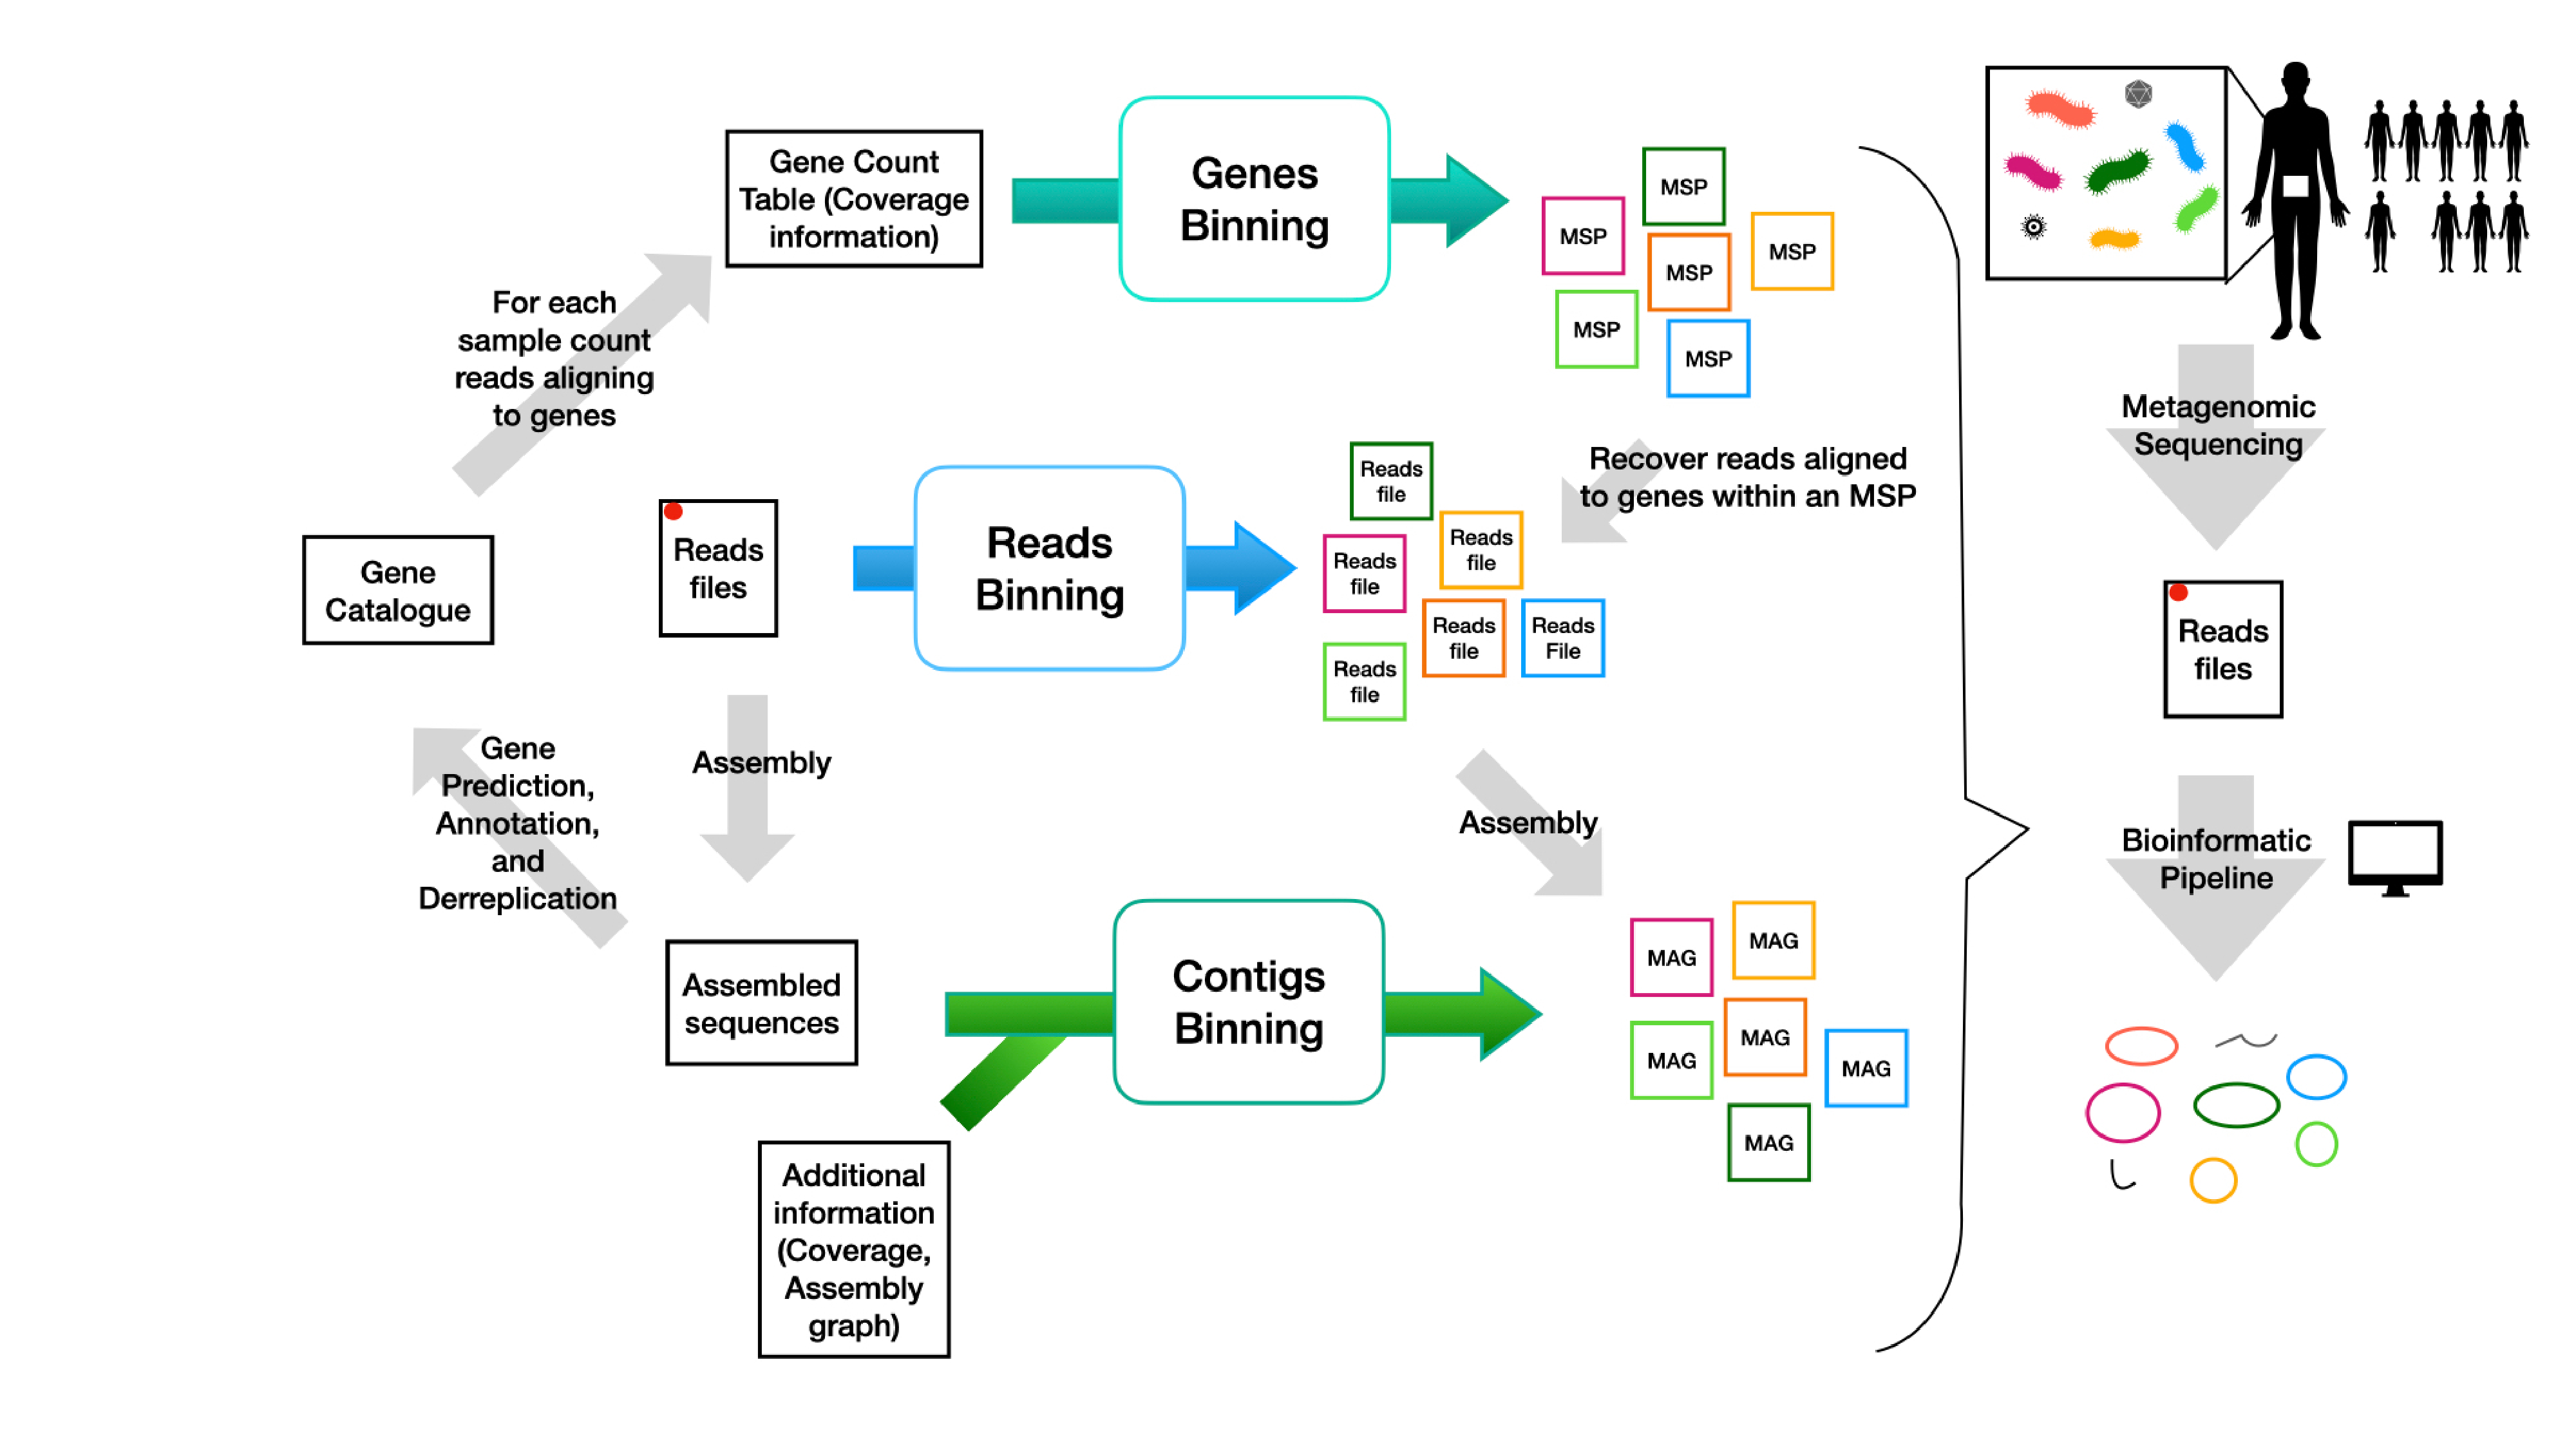
\includegraphics[scale=0.27]{figures/figure_binning_software.001.pdf}
\caption["Overview of the existing binning strategies."]{
	Overview of the existing binning strategies. a) Microbiome samples are collected and sequenced, the resulting sequences are processed, employing the existing binning strategies, which try to reconstruct the genome sequences from the original organisms. b) The scheme present a simplified workflow of the existing binning strategies, named contig-binning, reads-binning and genes-binning, represented as rounded rectangles in the middle of arrows. The star in the upper left indicates the entry point, simple arrows represent intermediate processing steps, black edge squares represent intermediate files, the color squares represent endpoint files. The binning strategies are not independent and can complement each other as shown by the dotted arrows.}
\label{Fsummary}
\end{figure}

\section{Background}
The explosion in popularity and success in the field of metagenomics over the last 25 years can be largely attributed to the advances in computing technologies.
An example of the outcomes of this can be found in the \gls{HMP}; a project that has been greatly improved the understanding of the microbiome flora involved in human health and disease \cite{turnbaugh2007human}.
These advances have brought with them greater demands for storage, \gls{CPU} time, and consequently more efficient algorithms.
The main function of binning tools is to reconstruct species/biological entities from metagenomic samples.  
Compared to amplicon, shotgun metagenome can provide functional gene profiles directly and reach a much higher resolution of taxonomic annotation.
However, due to the high demands on computational resources, cost, and expertise necessary to perform this analysis, researchers have historically been limited in their capacity to collect and analyse sequencing data.
As the cost of sequencing is rapidly falling, this burden has been significantly lessened.
Accurate, robust, and suitable binning methods are crucial for the proper interpretation of any metagenomic dataset.
Here we will briefly recapitulate recent binning algorithms and highlight some of the developments in the field, among them, the use of new algorithms and strategies employed to achieve the goal of identifying the organisms composing microbiome communities.

\section{Overview of recent methods for metagenomic binning}
\subsection{Progress in recent binning strategies}
A metagenomic sample is comprised of many organisms and the goal of binning is to reconstruct the sequences from each organism present in the original sample.
The majority of binning tools are oriented toward clustering contigs (contig-binning) into bins, which may represent the genome from a single biological entity/organism.
A \gls{MAG} is a single-taxon assembly based on one or more binned metagenomes that has been asserted to be a close representation to an individual genome that could match an already existing isolate or represent a novel isolate.
Current contig-binning tools are commonly reference free (i.e. they do not depend on reference sequences to perform clustering) and rely on coverage information and sequence composition.
Progress in contig-binning algorithms can be seen in the proposals to integrate new sources of information (for example, from scaffold-graphs (Binnacle \cite{Muralidharah2021binnacle}), paired-end reads (COCACOLA) \cite{Lu2016COCACOLA}, or 3D contact information (MetaTOR) \cite{Baudry2019Metator}) and state of the art algorithms in machine learning (CoCoNet, VAMB) \cite{nissenimproved, arisdakessian2021coconet}.
We also notice the development of Bin refinement tools (DAS-tool, Binning Refiner) that rely on the outputs from multiple contig-binning algorithms and combine them to produce better results \cite{Song2017Binningrefiner, sieber2018recovery}, and tools which allow visual inspection of bins \cite{Broeksema2017IcoVer, Laczny2017BusyBee}.
Binning of contigs have played a central role in software development in the field, a review on the benchmarking of binning algorithms was done by \citeNP{yue2020evaluating}. 
Beside contig-binning tools we can also distinguish read-binning tools and co-abundant-gene-binning tools.
The main purpose of read-binning tools is to pre-process reads into clusters for a posterior targeted assembly.
Here we find reference-free and non-reference-free tools, and tools designed for short-read or long-read sequencing technologies.
Among the binning tools developed in recent years, a subset of them are dedicated to cluster reads (read-binning) (MetaBBC-LR, BioBloom Tools, CLAME, LVQ-KNN, Meta VW, HirBin, MEGAN-LR) \cite{wickramarachchi2020metabcc, chu2014biobloom, benavides2018clame, belka2018lvq, vervier2016large, osterlund2017hirbin, huson2018megan}.

\subsubsection{Binning co-abundant genes}
Binning of co-abundant genes represents an alternative proposal to reconstruct species/biological entities from a set of metagenomic samples.
Co-abundant gene binning methods assumes that each gene coming from a shared chromosome will display proportional abundances across samples.
Therefore, if there are enough samples from a similar environment you can identify the sets of genes from a common organism of origin (MLGs Chameleon-clust 2012, CAGs and MGSs Canopy 2014, Markovclust-MGCs Karlsson 2013, \glspl{MSP} MSPminner 2018) \cite{karypis1999chameleon, plaza2019mspminer}.
The MSPminer software was developed to exploit this approach.
MSPminer introduced a robust proportionality measure to detect co-abundance but no necessarily co-occurrance.
This tool groups co-abundant genes into \glspl{MSP} and classifies genes within an \gls{MSP} as core, accessory and shared.
Core genes are present in all strains, accessory are present only in some, and the shared category applies for those genes which may be present in more than one \gls{MSP} due to horizontal transfer \cite{tettelin2005genome}.
Factors that impact directly on \gls{MSP} quality include sample composition, sequencing depth, and previous bioinforamtic steps to build the reference gene dataset and map the reads.
\glspl{MSP} can be used for taxonomic profiling of new samples from similar ecosystems at the species level, and also to compare strains between samples by building a presence/absence table of accessory genes and for biomarker discovery.
By binning contigs carrying genes from the same \gls{MSP} it is also possible to build a \gls{MAG}.

\subsubsection{Binning microbial genomes with deep learning}
The integration of deep learning techniques has revolutionised the field of metagenomics.
Deep learning approaches have benefitted from the rapid acceleration in GPU efficiency over the past few years.
The Software VAMB and CoCoNet constitute two such examples that employ deep learning for binning \cite{nissenimproved, arisdakessian2021coconet}.

The main novelty of VAMB is the application of the Deep Learning technique known as \gls{VAE}.
In this case, \glspl{VAE} learn how to integrate two data types, coabundance and k-mer composition.
The resulting latent representation is able to cluster better than either of the inputs alone.
In principle this technology is not limited by only two input data types.
VAMB also applies a "mulitsplit" approach whereby each cluster should correspond to an organism representation across samples and each bin in a cluster to a per-sample representation of the genome of that orgamisn.

The CoCoNet software uses deep learning and clustering to bin contigs into clusters representing species present in the samples.
The algorithm consists of two phases.
During the first phase, a neural network is trained to estimate the probability that two contigs arise from the same genome given their composition and coverage information.
The second use a heuristic to bin the contigs using the probabilities inferred in the first stage
An interesting feature in CoCoNet is it was trained on viral genomes. In the following section we discuss more about binning on viral genomes. 

\subsection{Binning of viral genomes}
Most binning algorithms are designed for prokariotic organisms leaving viruses out of the software scope.
In recent years the virome and its importance in health and disease has recognised.
CoCoNet uses deep leaning to model co-ocurrence of contigs from the same viral genome.
The network was optimized for diverse viral metagenomes, the network learns to model coverage variability within samples, a critical feature in viral metagenomes where DNA amplification methods are needed to increase input genetic material.
VirBin clusters contigs for genome reconstruction of viral strains, different strains within viral species may show different biological properties such as transmissibility or virulence. Composition based features are usually are not enough to separate haplotypes, VirBin receives contigs as inputs and outputs the estimated number of haplotypes via contig aligment and returns the contigs for each haplotype based on relative abundance distribution, when the contigs are long enough VirBin produce better results.
Newer strategies has been proposed and employed to reconstruct viral genomes from metagenomic samples, in a recent work \cite{nayfach2021metagenomic} a new compendium of 189680 DNA viruses from the human gut microbiome was produced.
In this work they use viral informative features including presence of viral protein families \cite{paez2016uncovering}, absence of non-viral families \cite{el2019pfam}, gene strand switch rate \cite{roux2005combined}, and the score produced from the VirFinder \cite{ren2017virfinder} software.

\subsection{Binning Pipelines}
Other advances in binning can be found in the integration of existing tools and software into bioinformatic pipelines.
These innovations allow the automatic complete processing of read samples into bins or the addition of extra processing steps to address specific biological questions or problems related to the sample of origin.
MetaWRAP is a modular pipeline ready to perform common tasks in metagenomic analysis, starting from read quality checks up to bin creation, refinement, reassembly quantification, taxonomic annotation and functional annotation.
MAGO pipeline integrates metagenome assembly, binning, bin improvement, bin quality check, bin functional annotation, and bin taxonomic annotation. 
SqueezeMeta also integrates external software to perform the complete analysis of metagenomic samples from sequences reading to \gls{MAG} construction and annotation \cite{tamames2019squeezemeta}
nf-mag supports both short and long reads, performs quality and adapter trimming, quality check,  performs assembly, binning, checks bin quality and assigns taxonomy \cite{ewels2020nf}.
Autometa was developed to deal with non-model Eukariotic host contamination and complex single metagenomes, the application integrate sequence homology, nucleotide composition, coverage and single-copy marker genes to separate microbial genomes from non model host genomes \cite{miller2019autometa}. 
Seqdex is a tool written in R which separates endosymbionts from their host sequences \cite{chiodi2019seqdechi}.
Their approach uses specific features in endosymbiotic systems to better solve this problem.
This tool combines partial taxonomic annotations obtained trough homology searches and sequence composition to predict the contig's organism of origin from host and its endosymbionts and helps the user to understand how effective is the classification.
Reproducibility, scalability, and ease of use from people with little computational experience are attractive features that pipelines for metagenomic analysis provide.

\section{Challenges in appropriate binning algorithm selection}
\begin{sidewaystable}
\begin{tiny}
\centering
\caption[Comparison of popular binning algorithms updated since 2017]{Comparison of popular binning algorithms updated since 2017.}
	\begin{tabular}{lrlllr}
\toprule
        Software/Algorithm &  Year &                                Description/purpose &                                  Comment/Highlight &                            Doi &  PubmedID \\
\midrule
                   CoCoNet &  2021 &    Deep learning tool for Viral Metagenome Binning &                          Reconstucts viral genomes & 10.1093/bioinformatics/btab213 &  33822891 \\
                  Binnacle &  2021 & Using scaffolds to improve Metagenomic bin quality &                  Incorporates scaffold information &      10.3389/fmicb.2021.638561 &  33717033 \\
                      VAMB &  2021 & Metagenome binning using deep variational autoe... &            Autoencoder algorithm, fast processing  &     10.1038/s41587-020-00777-4 &  33398153 \\
                phyloFlash &  2020 &                  ssrRNA profiling and MAG assembly & incorporates ssrRNA profiling info into MAG ass... &      10.1128/mSystems.00920-20 &  33109753 \\
                MetaBCC-LR &  2020 &                 Metagenomic binning for Long-Reads &      Suitable for Long Reads sequencing technology & 10.1093/bioinformatics/btaa441 &  32657364 \\
            BioBloom Tools &  2020 & Reads binning for targeted assembly, alignment ... & Data preparation for targeted assembly, using s... &        10.1073/pnas.1903436117 &  32641514 \\
                  GraphBin &  2020 & Refined binning of metagenomic contigs using as... &           Incorporates assembly graphs information & 10.1093/bioinformatics/btaa180 &  32167528 \\
                MetaSIPSim &  2020 & Simulating metagenomic stable isotope probing d... & Augment binning resolution with extra experimen... &      10.1186/s12859-020-3372-6 &  32000676 \\
                   MetaCon &  2019 & Unsupervised binning k-mers and coverage, focus... &                    Focus different lengths contigs &      10.1186/s12859-019-2904-4 &  31757198 \\
                    VirBin &  2019 &    Binning viral haplotypes from assembled contigs &                              Viral haplotypes MAGs &      10.1186/s12859-019-3138-1 &  31684876 \\
MAGO (*only tool pipeline) &  2019 &      Framework for Production and analysis of MAGs &                                           pipeline &          10.1093/molbev/msz237 &  31633780 \\
                    SeqDex &  2019 & Genome separation of Endosymbionts from mixed s... &                     Identification of endosymbiont &       10.3389/fgene.2019.00853 &  31608107 \\
                   MetaTOR &  2019 & High quality MAGs from mammalian guts using met... &                Incorporates 3D contact information &       10.3389/fgene.2019.00753 &  31481973 \\
                 MetaBAT 2 &  2019 & Adatptative binning algorithm for genome recons... & Eliminates manual parameter tuning from previou... &             10.7717/peerj.7359 &  31388474 \\
                   MetaBMF &  2019 & Scalable binning algorithm for large scale meta... &     Employs sample X contigs cf mapped read counts &  10.1093/bioinformatics/btz577 &  31347687 \\
               PolyCRACKER &  2019 & Method for partitioning polyploid sub genomes b... &                   Haplotypes for polyploid genomes &      10.1186/s12864-019-5828-5 &  31299888 \\
                  SolidBin &  2019 & Improving metagenome binning with semi-supervis... &                                                NaN &  10.1093/bioinformatics/btz253 &  30977806 \\
                  Autometa &  2019 & extraction of microbial genomes from individual... &                   Handles eukaryotic contamination &             10.1093/nar/gkz148 &  30838416 \\
    MLBP MrGBP (Algorithm) &  2019 & Signal processing method for alignment free met... & Alternative description of sequences designed f... &     10.1038/s41598-018-38197-9 &  30770850 \\
                     CLAME &  2018 & Aligment based algorithm allowed description of... &                          Aligment  based for reads &      10.1186/s12864-018-5191-y &  30537931 \\
     3D BH SNE (Algorithm) &  2018 &    Fuzzy binning of metagenomic sequence fragments & Horizontal gene transfer and regions of uncerta... &      10.1109/EMBC.2018.8512529 &  30440633 \\
                   LVQ-KNN &  2018 & Composition based RNA or DNA binning of short s... &                  Classify into DNA or RNA sequence & 10.1016/j.virusres.2018.10.002 &  30291874 \\
                  MSPminer &  2018 & Abundance based reconstitution of microbial pan... &                          Pan genome reconstitution &  10.1093/bioinformatics/bty830 &  30252023 \\
                 MetaWRAP* &  2018 & Flexible pipeline for genome resolved metagenom... &                    Hybrid bin extraction algorithm &      10.1186/s40168-018-0541-1 &  30219103 \\
                    MetaVW &  2018 & Large scale Machine Learning Sequence classific... &  Machine learning for reads based on Khmer profile &    10.1007/978-1-4939-8561-6\_2 &  30030800 \\
         Opal (algorithm*) &  2018 &    Metagenomic binning through low density binning & Improvement at higher taxonomic levels, discove... &  10.1093/bioinformatics/bty611 &  30010790 \\
                     BMC3C &  2018 & Binning contigs using codon usage sequence comp... &                        Add codon usage information &  10.1093/bioinformatics/bty519 &  29947757 \\
                AMBER tool &  2018 &                   Assessment of Metagenome Binners &                                                NaN &     10.1093/gigascience/giy069 &  29893851 \\
                  DAS Tool &  2018 &    Derreplication aggregation and scoring strategy &         Combines several binning algorithm results &      10.1038/s41564-018-0171-1 &  29807988 \\
                  MEGAN-LR &  2018 &              Long Read/ contigs taxonomic binning  & Aligment of long reads against reference sequences &      10.1186/s13062-018-0208-7 &  29678199 \\
                     CoMet &  2018 & Binning workflow using contain coverage and com... & Single sample, include gc content  and 4mer fre... &      10.1186/s12859-017-1967-3 &  29297295 \\
                         ? &  2017 & Metagenomic binning and association of plasmids... & Plasmid banning at strain level using methylati... &               10.1038/nbt.4037 &  29227468 \\
                   MetaGen &  2017 & reference-free learning with multiple metagenom... &                          Requires multiple samples &      10.1186/s13059-017-1323-y &  28974263 \\
            d2sBin add onn &  2017 & Improved formula for calculate oligonucleotide ... & Math formula to calculate oligo sequence dissim... &      10.1186/s12859-017-1835-1 &  28931373 \\
               BusyBee Web &  2017 &     Bootstrapped supervises binning and annotation &     2d interactive scatterplots supervised binning &             10.1093/nar/gkx348 &  28472498 \\
                    ICoVer &  2017 & Interactive visualisation tool for verification... &                     Interactive visualisation tool &     10.1186/s12859-017-1653-5" &  28464793 \\
                   HirBin* &  2017 & High resolution identification of differentiall... & Supervised annotation, unsupervised clustering ... &      10.1186/s12864-017-3686-6 &  28431529 \\
                 BinSanity &  2017 & Unsupervised clustering using coverage and affi... &                Reduce bias for high/low abundance  &             10.7717/peerj.3035 &  28289564 \\
          Binning\_refinner &  2017 & Improve genome bins through the combination of ... &        Combination of different binning algorithms &  10.1093/bioinformatics/btx086 &  28186226 \\
               IFCM add on &  2016 &        Improved binning using Fuzzy C-Means Method &  Add estimated distribution of real genome lengths &      10.1109/TCBB.2016.2576452 &  27295684 \\
                  COCACOLA &  2016 & binning contigs using composition, read coverag... &    Adds paired end read and coaligment information &  10.1093/bioinformatics/btw290 &  27256312 \\
                GroopM (2) &  2014 & Tool for automatic recovery of population genom... & Adds differential coverage to complement compos... &              10.7717/peerj.603 &  25289188 \\
\bottomrule
\end{tabular}

\label{Tbinningsoftware}
\end{tiny}
\end{sidewaystable}
A number of aspects should be considered when performing binning analysis on metagenomic samples.
Computational resources available, sequencing technology, number of samples, and the sample's source are important factors to consider.
Some tools employ more resources than others, and some perform better under specific circumstances (as reviewed by \citeNP{yue2020evaluating}).
If you are dealing with a large number of samples, a tool like MetaBMF \cite{Xing2017MetaGen, Ma2019MetaBMF} or a gene-binning strategy could be taken into consideration.
Tools such as CoMet were built around single sample binning \cite{herath2017comet}.
Long read sequence technology is gaining momentum and some tools also integrate the characteristic features generated with this technology.
The environment under study also play an important role for binning.
Sometimes there exists host organisms whose genome sequences would be removed before starting the analysis.
The environment also has a profound effect on the sample's diversity with samples that have greater diversity requiring greater sequencing depth making binning more difficult.
It is also difficult for binning tools to discern between similar strains within the same sample.  
It is also worth mentioning that there is no mutual exclusivity between the currently available tools and it is possible to benefit from the relative advantages each has to offer and merge the results depending of the aim of the study.
Besides binning, other types of metagenomic analysis can be performed on microbiomes.
Recent reviews provide an overview of the complete process and practical guides to apply available software \cite{breitwieser2019review}.  

\section{Conclusion}
Popularity and successes of metagenomic binning have accelerated in the last ten years.
Current limitations that still remain include the difficulty in classifying similar strains within samples.
They additionally do not perform well assigning 16S sequences to bins likely due to the high copy number of these sequences within a genome.
As binning has been focused mainly in prokariotic organisms, binning of organisms outside prokariotes need more development.
Although there have been signifiance advances in the characterisation of viral genomes as of late \cite{nayfach2021metagenomic}, the huge diversity in viral genomes still poses a challenge for current methodologies.
The continuously increasing number of sequences available require more efficient/faster algorithms and new strategies to reconstruct single organisms from environmental samples.
However, with the breakneck pace of technological advancements in computing resources, this requirement is sure to be met and will pave the way for greater insights into the microbial world.
With the integration of Machine learning algorithms into binning, we expect to see significant developments in the near future.

\bibliography{library}
\section*{Acknowledgements}
We thank members of Sysbiomelab and Sysmedicine (Mardinoglu lab) for their invaluable support during this work. This work was funded by KTH Royal Institute of Technology and School of Engineering Sciences in Chemistry,
Biotechnology and Health (CBH).

\end{document}
